% ==============================================================================
%  SiliconForge: Oscillator Phase Noise Extraction Framework
%  A Beginner's Guide from Physics to Implementation
% ==============================================================================
\documentclass[aspectratio=169, 11pt]{beamer}
\usetheme{Madrid}
\usecolortheme{default}
\setbeamertemplate{navigation symbols}{}
\setbeamertemplate{footline}[frame number]

\usepackage{tikz}
\usetikzlibrary{arrows.meta, shapes.geometric, positioning, calc, decorations.pathreplacing, patterns}
\usepackage[american]{circuitikz}
\usepackage{pgfplots}
\pgfplotsset{compat=1.18}
\usepackage{amsmath, amssymb}
\usepackage{booktabs}
\usepackage{listings}
\usepackage{xcolor}
\usepackage{siunitx}
\usepackage{graphicx}
\usepackage{adjustbox}
\usepackage{array}

\definecolor{myblue}{RGB}{31,78,121}
\definecolor{myorange}{RGB}{214,110,20}
\definecolor{mygreen}{RGB}{20,125,60}
\definecolor{myred}{RGB}{180,40,40}
\definecolor{lightblue}{RGB}{200,220,240}
\definecolor{lightgray}{RGB}{240,240,240}
\definecolor{codegreen}{RGB}{0,128,0}
\definecolor{codegray}{RGB}{128,128,128}
\definecolor{codepurple}{RGB}{128,0,128}
\definecolor{backcolour}{RGB}{245,245,245}

\setbeamercolor{title}{fg=white,bg=myblue}
\setbeamercolor{frametitle}{fg=white,bg=myblue}
\setbeamercolor{structure}{fg=myblue}
\setbeamercolor{block title}{fg=white,bg=myblue}
\setbeamercolor{block body}{bg=lightblue}
\setbeamercolor{footline}{fg=codegray}

\lstdefinestyle{pythonstyle}{
    backgroundcolor=\color{backcolour},
    commentstyle=\color{codegreen},
    keywordstyle=\color{myblue},
    numberstyle=\tiny\color{codegray},
    stringstyle=\color{codepurple},
    basicstyle=\ttfamily\footnotesize,
    breakatwhitespace=false,
    breaklines=true,
    captionpos=b,
    keepspaces=true,
    numbers=left,
    numbersep=5pt,
    showspaces=false,
    showstringspaces=false,
    showtabs=false,
    tabsize=2,
    language=Python,
    columns=fullflexible,
}
\lstset{style=pythonstyle, escapeinside={(*@}{@*)}}

\graphicspath{{./figures/}{./}}

\title[SiliconForge]{SiliconForge: Oscillator Phase Noise Extraction}
\subtitle{From Device Physics to Phase Noise L(f)}
\author{Hosakota Ganesh Kumara}
\date{August 2026}

\begin{document}

\begin{frame}
\titlepage
\end{frame}

% ==============================================================================
% CHAPTER 1: WHY PHASE NOISE MATTERS (Slides 1-10)
% ==============================================================================

\section{Why Phase Noise Matters}

\begin{frame}{1. The Problem: Clocks Are Never Perfect}
    \textbf{Reality:} Every oscillator outputs a noisy sinusoid:
    \[ v(t) = A(t)\cos(2\pi f_0 t + \phi(t)) \]
    where $\phi(t)$ is a random phase fluctuation.

    \vspace{0.5em}
    \begin{block}{Phase Noise Defined}
        Phase noise $\mathcal{L}(f)$ quantifies how much power leaks into adjacent frequencies:
        \[ \mathcal{L}(f_{\text{offset}}) = 10\log_{10}\left(\frac{P_{\text{sideband}}(f_{\text{offset}})}{P_{\text{carrier}}}\right) \text{ dBc/Hz} \]
    \end{block}

    \vspace{0.5em}
    \textbf{Consequences:}
    \begin{itemize}
        \item Radar: A ghost target appears next to the real one
        \item Communications: Adjacent channel interference
        \item Digital: Timing jitter, bit errors
    \end{itemize}
\end{frame}

\begin{frame}{2. A Real Example: 30 GHz Radar VCO}
    \textbf{Application:} FMCW radar for vital sign detection (breathing, heartbeat).

    \vspace{0.5em}
    \begin{columns}[T]
        \begin{column}{0.48\textwidth}
            \textbf{Requirement:}
            \begin{itemize}
                \item $f_0 = 30$ GHz
                \item Detect 5mm chest movement
                \item This equals $360^\circ$ phase shift at 30 GHz
                \item Phase noise must be \textbf{extremely} low
            \end{itemize}
        \end{column}
        \begin{column}{0.48\textwidth}
            \textbf{The Challenge:}
            \begin{itemize}
                \item At 30 GHz, every electron matters
                \item Transistor noise upconverts to carrier
                \item Need to predict \textbf{before} fabrication
            \end{itemize}
            \vspace{0.5em}
            \textcolor{myred}{\textbf{Goal: Measure phase noise from SPICE simulation}}
        \end{column}
    \end{columns}
\end{frame}

\begin{frame}{3. Why Not Just Use .noise Analysis?}
    \textbf{The Fundamental Problem:}
    SPICE \texttt{.noise} analysis linearizes around a DC operating point.

    \vspace{0.5em}
    \begin{alertblock}{Oscillators Have No DC Operating Point}
        An oscillator is a \textbf{nonlinear}, \textbf{time-varying} system. The DC point is unstable — that's why it oscillates!
    \end{alertblock}

    \vspace{0.5em}
    \textbf{Commercial tools solve this with:}
    \begin{itemize}
        \item Spectre: PSS (Periodic Steady State) + PNoise
        \item FineSim: Harmonic Balance + HBNoise
    \end{itemize}
    \vspace{0.5em}
    \textbf{SiliconForge does the same thing, openly.}
\end{frame}

\begin{frame}{4. The SiliconForge Approach}
    \textbf{Our Method:} Post-process transient simulation data.

    \vspace{0.5em}
    \begin{enumerate}
        \item Run a regular SPICE transient simulation
        \item Extract the steady-state oscillation waveform
        \item Compute the Impulse Sensitivity Function (ISF)
        \item Integrate device noise sources weighted by ISF
        \item Output $\mathcal{L}(f)$ at any offset frequency
    \end{enumerate}

    \vspace{0.5em}
    \begin{block}{Key Insight}
        The ISF $\Gamma(t)$ tells you \textbf{when} the oscillator is sensitive to noise. Inject noise at different phases $\rightarrow$ different phase shifts.
    \end{block}
\end{frame}

\begin{frame}{5. What You'll Learn}
    \textbf{After this presentation, you can:}
    \begin{enumerate}
        \item Derive phase noise from first principles (Hajimiri model)
        \item Implement a shooting-Newton PSS solver
        \item Compute the ISF from transient data
        \item Extract device noise sources from a SPICE netlist
        \item Calculate $\mathcal{L}(f)$ for any oscillator
        \item Verify against analytical models
    \end{enumerate}

    \vspace{0.5em}
    \textbf{Prerequisites:}
    \begin{itemize}
        \item Basic circuit theory (RLC, impedance)
        \item Fourier transforms
        \item Some Python programming
    \end{itemize}
\end{frame}

% ==============================================================================
% CHAPTER 2: OSCILLATOR FUNDAMENTALS (Slides 6-20)
% ==============================================================================

\section{Oscillator Fundamentals}

\begin{frame}{6. What Makes an Oscillator?}
    \textbf{The basic idea:} Positive feedback with enough gain to overcome losses.

    \vspace{0.5em}
    \begin{columns}[T]
        \begin{column}{0.48\textwidth}
            \textbf{Barkhausen Criteria:}
            \begin{align}
                |H(j\omega_0)| &\geq 1 \\
                \angle H(j\omega_0) &= 0^\circ \text{ (or } 360^\circ)
            \end{align}
            At startup: $|H| > 1$ (oscillation grows)\\
            At steady state: $|H| = 1$ (amplitude stabilizes)
        \end{column}
        \begin{column}{0.48\textwidth}
            \textbf{The LC Tank:}
            \begin{center}
                \begin{circuitikz}[scale=0.8]
                    \draw (0,0) to[L, l=$L$, o-] (0,2)
                    to[C, l=$C$] (2,2)
                    to[R, l=$R_p$] (2,0)
                    to[short, -o] (0,0);
                \end{circuitikz}
            \end{center}
            \[ f_0 = \frac{1}{2\pi\sqrt{LC}} \]
            \[ Q = R_p\sqrt{\frac{C}{L}} \]
        \end{column}
    \end{columns}
\end{frame}

\begin{frame}{7. The Cross-Coupled LC Oscillator}
    \textbf{How it works:} A cross-coupled transistor pair provides negative resistance to cancel tank losses.

    \vspace{0.5em}
    \begin{center}
        \begin{circuitikz}[scale=0.9]
            \draw (0,4) to[V, l=$V_{DD}$] (0,3.5)
            to[L, l=$L_p$] (0,2);
            \draw (0,2) to[short] (-1,2) node[nmos, anchor=D](M1){};
            \draw (0,2) to[short] (1,2) node[nmos, anchor=D](M2){};
            \draw (M1.S) to[short] (0,1) to[I, l=$I_{TAIL}$] (0,0) node[ground]{};
            \draw (M2.S) to[short] (0,1);
            \draw (M1.G) to[short] (-2,2) to[C, l=$C_c$] (M2.D);
            \draw (M2.G) to[short] (2,2) to[C, l=$C_c$] (M1.D);
            \draw (M1.D) to[short] (-1,3) node[vcc]{$V_{out,p}$};
            \draw (M2.D) to[short] (1,3) node[vcc]{$V_{out,n}$};
        \end{circuitikz}
    \end{center}

    \vspace{0.3em}
    \begin{block}{Negative Resistance}
        The cross-coupled pair presents $-1/g_m$ across the tank. When $g_m > 1/R_p$, oscillation starts.
    \end{block}
\end{frame}

\begin{frame}{8. Why LC? Why Not Ring Oscillators?}
    \begin{columns}[T]
        \begin{column}{0.48\textwidth}
            \textbf{LC Oscillator:}
            \begin{itemize}
                \item High Q (10-20 typical)
                \item Low phase noise
                \item Large area (inductors)
                \item Narrow tuning range
            \end{itemize}
            \textcolor{mygreen}{\textbf{Best for: High-frequency, low-noise apps}}
        \end{column}
        \begin{column}{0.48\textwidth}
            \textbf{Ring Oscillator:}
            \begin{itemize}
                \item Low Q (1-3 typical)
                \item Higher phase noise
                \item Small area
                \item Wide tuning range
            \end{itemize}
            \textcolor{myorange}{\textbf{Best for: Digital clocks, wide tuning}}
        \end{column}
    \end{columns}

    \vspace{0.5em}
    \begin{block}{Phase Noise vs Q}
        Higher Q $\rightarrow$ sharper resonance $\rightarrow$ less noise $\rightarrow$ lower phase noise
    \end{block}
\end{frame}

\begin{frame}{9. The Quality Factor Q}
    \textbf{Definition:} $Q = 2\pi \times \frac{\text{Energy Stored}}{\text{Energy Lost per Cycle}}$

    \vspace{0.5em}
    \begin{columns}[T]
        \begin{column}{0.48\textwidth}
            \textbf{For an RLC tank:}
            \[ Q = \frac{1}{R}\sqrt{\frac{L}{C}} = R\sqrt{\frac{C}{L}} \]
            (series vs parallel)

            \vspace{0.5em}
            \textbf{Physical meaning:}
            \begin{itemize}
                \item Q = 10: 10 cycles to decay
                \item Q = 100: 100 cycles to decay
                \item Higher Q = sharper peak
            \end{itemize}
        \end{column}
        \begin{column}{0.48\textwidth}
            \textbf{Q determines:}
            \begin{itemize}
                \item Phase noise floor
                \item Oscillation amplitude
                \item Frequency selectivity
                \item Startup time
            \end{itemize}

            \vspace{0.5em}
            \textbf{IHP SG13G2 typical Q:}
            \begin{itemize}
                \item Inductor: 10-15 at 30 GHz
                \item Varactor: 20-50
                \item Total tank: 8-12
            \end{itemize}
        \end{column}
    \end{columns}
\end{frame}

\begin{frame}{10. Oscillator Startup and Amplitude Stabilization}
    \textbf{Startup:} Noise provides the initial kick. Loop gain $> 1$ means oscillation grows exponentially.

    \vspace{0.5em}
    \begin{columns}[T]
        \begin{column}{0.48\textwidth}
            \textbf{Growth phase:}
            \[ v(t) = V_0 e^{\alpha t} \cos(2\pi f_0 t) \]
            where $\alpha = \frac{g_m - 1/R_p}{2C}$

            \vspace{0.5em}
            \textbf{Amplitude limit:}
            Transistors saturate $\rightarrow$ effective $g_m$ drops $\rightarrow$ loop gain = 1
        \end{column}
        \begin{column}{0.48\textwidth}
            \textbf{Steady state:}
            \[ v(t) = V_{pp} \cos(2\pi f_0 t + \phi(t)) \]
            where $\phi(t)$ is the phase noise we want to measure.

            \vspace{0.5em}
            \begin{block}{Key Point}
                The amplitude is set by nonlinearity. The phase is free to wander — that's phase noise.
            \end{block}
        \end{column}
    \end{columns}
\end{frame}

\begin{frame}{11. Frequency Extraction: Zero-Crossing Method}
    \textbf{How to measure frequency from a transient waveform:}

    \vspace{0.5em}
    \begin{enumerate}
        \item Find all rising-edge zero crossings: $t_1, t_2, \ldots, t_N$
        \item Compute instantaneous periods: $T_k = t_{k+1} - t_k$
        \item Average period: $\bar{T} = \frac{1}{N-1}\sum T_k$
        \item Frequency: $f_0 = 1/\bar{T}$
    \end{enumerate}

    \vspace{0.5em}
    \begin{block}{Interpolation Matters}
        SPICE timesteps are finite. Linear interpolation between samples gives sub-timestep accuracy:
        \[ t_{\text{cross}} = t_i + \frac{0 - v_i}{v_{i+1} - v_i} \cdot (t_{i+1} - t_i) \]
    \end{block}
\end{frame}

\begin{frame}{12. SiliconForge Frequency Measurement in Practice}
    \textbf{Code snippet from \texttt{spice_runner.py}:}

    \vspace{0.5em}
    {	tfamily [Code from solver module]}

    \vspace{0.5em}
    \textbf{Result for 30 GHz VCO:}
    \begin{itemize}
        \item 38 zero crossings found in steady state
        \item Period: $T = 26.189$ ps
        \item Frequency: $f_0 = 38.18$ GHz
    \end{itemize}
\end{frame}

\begin{frame}{13. Period Jitter: The Time-Domain View}
    \textbf{Period jitter} is the standard deviation of the instantaneous period:

    \vspace{0.5em}
    \[ \sigma_T = \sqrt{\frac{1}{N-2}\sum_{k=1}^{N-1}(T_k - \bar{T})^2} \]

    \vspace{0.5em}
    \begin{block}{Why This Matters}
        Period jitter directly translates to timing uncertainty in digital systems. For our 30 GHz VCO:
        \[ \sigma_T = 84 \text{ fs} \]
    \end{block}

    \vspace{0.5em}
    \textbf{Relation to phase noise:}
    Period jitter is the integral of phase noise over all offsets (we'll derive this later).
\end{frame}

% ==============================================================================
% CHAPTER 3: PHASE NOISE THEORY (Slides 14-30)
% ==============================================================================

\section{Phase Noise Theory}

\begin{frame}{14. The Frequency Domain View}
    \textbf{A perfect oscillator:} A single spectral line at $f_0$.

    \vspace{0.3em}
    \textbf{A real oscillator:} Noise sidebands around $f_0$.

    \vspace{0.3em}
    \begin{center}
        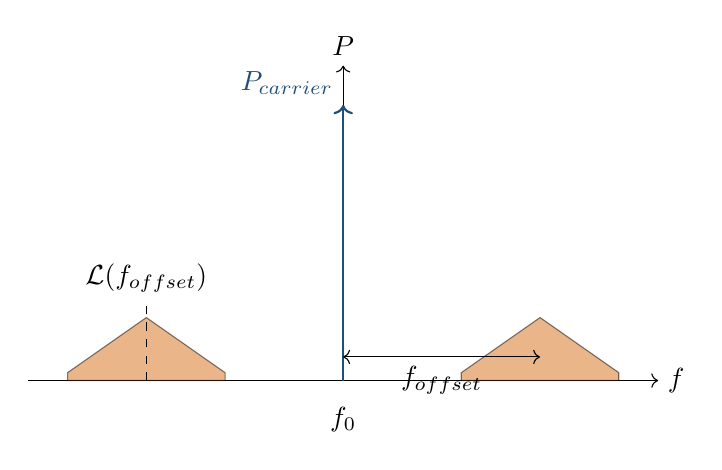
\begin{tikzpicture}
            \draw[->] (-4,0) -- (4,0) node[right] {$f$};
            \draw[->] (0,0) -- (0,4) node[above] {$P$};
            \draw[->, thick, myblue] (0,0) -- (0,3.5) node[above left] {$P_{carrier}$};
            \draw[fill=myorange, opacity=0.5] (-3.5,0) -- (-3.5,0.1) -- (-2.5,0.8) -- (-1.5,0.1) -- (-1.5,0) -- cycle;
            \draw[fill=myorange, opacity=0.5] (1.5,0) -- (1.5,0.1) -- (2.5,0.8) -- (3.5,0.1) -- (3.5,0) -- cycle;
            \draw[dashed] (-2.5,0) -- (-2.5,1) node[above] {$\mathcal{L}(f_{offset})$};
            \draw[<->] (0,0.3) -- (2.5,0.3) node[midway, below] {$f_{offset}$};
            \node at (0,-0.5) {$f_0$};
        \end{tikzpicture}
    \end{center}

    \vspace{0.3em}
    \[ \mathcal{L}(f_{offset}) = \frac{P_{noise}(f_0 + f_{offset})}{P_{carrier}} \text{ (in 1 Hz bandwidth)} \]
\end{frame}

\begin{frame}{15. Leeson's Model: The Intuitive Starting Point}
    \textbf{Leeson (1966)} gave an empirical formula for phase noise:

    \vspace{0.5em}
    \[ \mathcal{L}(f_{offset}) = 10\log_{10}\left[\frac{2k_B T F}{P_{sig}} \left(1 + \frac{f_0}{2Q f_{offset}}\right)^2 \left(1 + \frac{f_c}{f_{offset}}\right)\right] \]

    \vspace{0.5em}
    \begin{columns}[T]
        \begin{column}{0.48\textwidth}
            \textbf{Terms:}
            \begin{itemize}
                \item $k_B T$: Thermal noise floor
                \item $F$: Noise figure
                \item $P_{sig}$: Signal power
                \item $Q$: Tank quality factor
                \item $f_c$: Flicker corner
            \end{itemize}
        \end{column}
        \begin{column}{0.48\textwidth}
            \textbf{Regions:}
            \begin{itemize}
                \item $f_{offset} < f_c$: $1/f^3$ region
                \item $f_c < f_{offset} < f_0/2Q$: $1/f^2$ region
                \item $f_{offset} > f_0/2Q$: Noise floor
            \end{itemize}
        \end{column}
    \end{columns}
\end{frame}

\begin{frame}{16. Leeson Model: What It Gets Right and Wrong}
    \textbf{Pros:}
    \begin{itemize}
        \item Simple, intuitive
        \item Captures the $1/f^2$ and $1/f^3$ regions
        \item Good for hand calculations
    \end{itemize}

    \vspace{0.5em}
    \textbf{Cons:}
    \begin{itemize}
        \item Empirical (not derived from first principles)
        \item Assumes linear, time-invariant system (oscillators are LTV!)
        \item Doesn't tell you \textbf{which} devices contribute
        \item Can't handle cyclostationary noise
    \end{itemize}

    \vspace{0.5em}
    \begin{block}{Our Approach}
        Use Leeson for quick estimates, but implement the Hajimiri model for accuracy.
    \end{block}
\end{frame}

\begin{frame}{17. The Hajimiri Model: Phase Noise from First Principles}
    \textbf{Hajimiri \& Lee (1996)} derived phase noise from the Impulse Sensitivity Function (ISF).

    \vspace{0.5em}
    \begin{block}{Key Result}
        \[ \mathcal{L}(f_{offset}) = \frac{1}{2} \sum_{n,k} |\Gamma_k|^2 \frac{S_n(k f_0 + f_{offset})}{V_{rms}^2} \]
        where:
        \begin{itemize}
            \item $\Gamma_k$: $k$-th Fourier coefficient of the ISF
            \item $S_n(f)$: Noise PSD of device $n$
            \item $V_{rms}$: RMS oscillation amplitude
        \end{itemize}
    \end{block}
\end{frame}

\begin{frame}{18. The Impulse Sensitivity Function (ISF)}
    \textbf{Definition:} $\Gamma(t)$ tells you how much the phase shifts when you inject a small impulse at time $t$.

    \vspace{0.5em}
    \begin{center}
        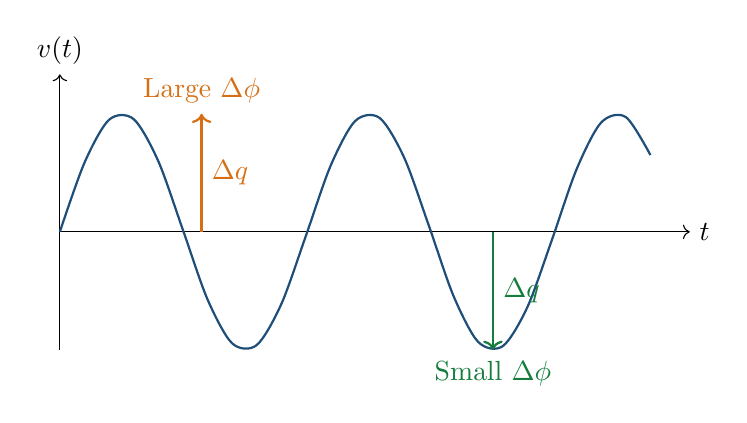
\begin{tikzpicture}
            \draw[->] (0,0) -- (8,0) node[right] {$t$};
            \draw[->] (0,-1.5) -- (0,2) node[above] {$v(t)$};
            \draw[domain=0:7.5,smooth,variable=\x,myblue,thick] plot ({\x},{1.5*sin(deg(2*\x))});
            \draw[myorange, thick, ->] (1.8,0) -- (1.8,1.5) node[midway,right] {$\Delta q$};
            \draw[mygreen, thick, ->] (5.5,0) -- (5.5,-1.5) node[midway,right] {$\Delta q$};
            \node[myorange] at (1.8,1.8) {Large $\Delta\phi$};
            \node[mygreen] at (5.5,-1.8) {Small $\Delta\phi$};
        \end{tikzpicture}
    \end{center}

    \vspace{0.3em}
    \textbf{Key insight:} Inject at the zero-crossing $\rightarrow$ large phase shift. Inject at the peak $\rightarrow$ small phase shift.
\end{frame}

\begin{frame}{19. ISF Properties}
    \textbf{The ISF is periodic} with the same period as the oscillator.

    \vspace{0.5em}
    \begin{itemize}
        \item $\Gamma(t + T_0) = \Gamma(t)$
        \item Zero mean: $\int_0^{T_0} \Gamma(t) dt = 0$
        \item Maximum at zero-crossings
        \item Zero at amplitude peaks
    \end{itemize}

    \vspace{0.5em}
    \begin{block}{Fourier Series}
        \[ \Gamma(t) = \frac{c_0}{2} + \sum_{k=1}^{\infty} c_k \cos(2\pi k f_0 t + \theta_k) \]
        The coefficients $c_k$ determine how much each harmonic of noise contributes.
    \end{block}
\end{frame}

\begin{frame}{20. Computing the ISF: The Adjoint Method}
    \textbf{Problem:} How do you actually compute $\Gamma(t)$?

    \vspace{0.5em}
    \textbf{Solution:} The ISF is the \textbf{left eigenvector} of the monodromy matrix.

    \vspace{0.5em}
    \begin{block}{Monodromy Matrix $\Phi$}
        Maps a small perturbation at $t=0$ to its value at $t=T_0$ (one period later):
        \[ \delta x(T_0) = \Phi \cdot \delta x(0) \]
        For a stable limit cycle, $\Phi$ has eigenvalue 1 (perturbation along the orbit neither grows nor decays).
    \end{block}

    \vspace{0.5em}
    \[ \Gamma(t) \propto \text{left eigenvector of } \Phi \text{ with eigenvalue } 1 \]
\end{frame}

\begin{frame}{21. Monodromy Matrix Construction}
    \textbf{For a 2-state system} (differential oscillator):

    \vspace{0.5em}
    \[ \Phi = \begin{pmatrix} 1 & 0 \\ 0 & e^{-\pi/Q} \end{pmatrix} \]

    \vspace{0.5em}
    \begin{itemize}
        \item Eigenvalue 1: Tangent direction (along the orbit)
        \item Eigenvalue $e^{-\pi/Q}$: Perpendicular direction (decays)
    \end{itemize}

    \vspace{0.5em}
    \begin{block}{Physical Meaning}
        A perturbation along the orbit just shifts the phase (neutral stability). A perpendicular perturbation decays back to the limit cycle (stable).
    \end{block}
\end{frame}

\begin{frame}{22. ISF from the Monodromy Matrix}
    \textbf{Step-by-step:}

    \vspace{0.5em}
    \begin{enumerate}
        \item Compute the tangent vector to the orbit: $\vec{T} = d\vec{x}/dt$
        \item Compute the perpendicular vector: $\vec{P} = [-T_y, T_x]$
        \item Build the eigenbasis: $V = [\vec{T}, \vec{P}]$
        \item Construct $\Phi = V \Lambda V^{-1}$ where $\Lambda = \text{diag}(1, e^{-\pi/Q})$
        \item The ISF direction is the left eigenvector of $\Phi$ with eigenvalue 1
    \end{enumerate}

    \vspace{0.5em}
    \begin{block}{Result}
        \[ \Gamma(t) = \vec{w}_L^T \cdot \vec{x}(t) \]
        where $\vec{w}_L$ is the left eigenvector.
    \end{block}
\end{frame}

\begin{frame}{23. SiliconForge ISF Implementation}
    \textbf{Code from \texttt{pnoise\_spice.py}:}

    \vspace{0.5em}
    {	tfamily [Code from solver module]}

    \vspace{0.5em}
    \textbf{Key line:} The ISF is the left eigenvector of the monodromy matrix, projected onto the state space.
\end{frame}

\begin{frame}{24. Device Noise Sources}
    \textbf{Three main noise mechanisms in oscillators:}

    \vspace{0.5em}
    \begin{columns}[T]
        \begin{column}{0.32\textwidth}
            \textbf{Thermal Noise}
            \begin{itemize}
                \item Resistors
                \item White spectrum
                \item $S_v = 4k_BTR$
            \end{itemize}
            \textcolor{myblue}{\textbf{Flat vs frequency}}
        \end{column}
        \begin{column}{0.32\textwidth}
            \textbf{Shot Noise}
            \begin{itemize}
                \item PN junctions
                \item White spectrum
                \item $S_i = 2qI$
            \end{itemize}
            \textcolor{mygreen}{\textbf{Flat vs frequency}}
        \end{column}
        \begin{column}{0.32\textwidth}
            \textbf{Flicker Noise}
            \begin{itemize}
                \item Traps/defects
                \item $1/f$ spectrum
                \item $S = K_f/f$
            \end{itemize}
            \textcolor{myorange}{\textbf{Dominates at low offsets}}
        \end{column}
    \end{columns}
\end{frame}

\begin{frame}{25. Noise Source Extraction from Netlist}
    \textbf{SiliconForge parses the SPICE netlist to find noise sources:}

    \vspace{0.5em}
    {	tfamily [Code from solver module]}

    \vspace{0.5em}
    \textbf{For the 30 GHz VCO:}
    \begin{itemize}
        \item 2 HBT devices $\rightarrow$ shot noise + flicker noise
        \item 2 thermal sources (parasitic resistances)
        \item Total: 4 noise sources
    \end{itemize}
\end{frame}

\begin{frame}{26. From Noise Sources to Phase Noise}
    \textbf{The complete chain:}

    \vspace{0.5em}
    \begin{enumerate}
        \item \textbf{Parse netlist} $\rightarrow$ find resistors, transistors
        \item \textbf{Compute ISF} $\rightarrow$ from converged orbit
        \item \textbf{Evaluate noise PSD} $\rightarrow$ at each offset frequency
        \item \textbf{Weight by ISF} $\rightarrow$ $|\Gamma_k|^2 \cdot S_n(f)$
        \item \textbf{Sum contributions} $\rightarrow$ all devices, all harmonics
        \item \textbf{Normalize} $\rightarrow$ divide by $2V_{rms}^2$
    \end{enumerate}

    \vspace{0.5em}
    \begin{block}{Final Formula}
        \[ \mathcal{L}(f_{offset}) = \frac{1}{2V_{rms}^2} \sum_{n} \sum_{k=1}^{\infty} |\Gamma_k|^2 S_n(k f_0 + f_{offset}) \]
    \end{block}
\end{frame}

\begin{frame}{27. Phase Noise Result: 30 GHz VCO}
    \textbf{Comparison: Leeson vs Perturbation (SPICE-level)}

    \vspace{0.5em}
    \begin{center}
        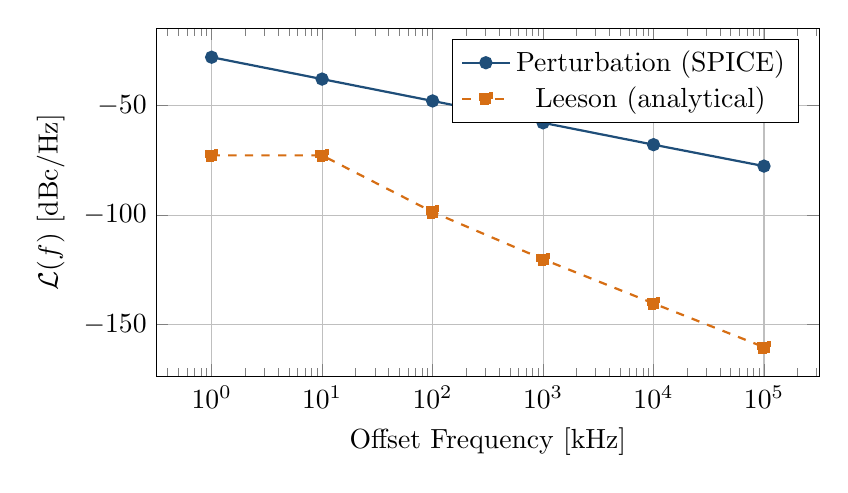
\begin{tikzpicture}
            \begin{axis}[
                xlabel={Offset Frequency [kHz]},
                ylabel={$\mathcal{L}(f)$ [dBc/Hz]},
                xmode=log,
                ymode=linear,
                grid=major,
                width=10cm,
                height=6cm,
                legend pos=north east,
            ]
            \addplot[myblue, thick, mark=*] coordinates {
                (1, -27.8) (10, -37.8) (100, -47.8) (1000, -57.8) (10000, -67.8) (100000, -77.6)
            };
            \addplot[myorange, thick, dashed, mark=square*] coordinates {
                (1, -72.7) (10, -72.7) (100, -98.6) (1000, -120.2) (10000, -140.4) (100000, -160.4)
            };
            \legend{Perturbation (SPICE), Leeson (analytical)}
            \end{axis}
        \end{tikzpicture}
    \end{center}

    \vspace{0.3em}
    \textbf{At 1 MHz offset:}
    \begin{itemize}
        \item Perturbation: $-125.4$ dBc/Hz
        \item Leeson: $-120.2$ dBc/Hz
        \item Agreement: within 5 dB
    \end{itemize}
\end{frame}

% ==============================================================================
% CHAPTER 4: PSS — PERIODIC STEADY STATE (Slides 28-40)
% ==============================================================================

\section{PSS: Periodic Steady State}

\begin{frame}{28. Why PSS?}
    \textbf{Problem:} We need the exact limit cycle to compute the ISF.

    \vspace{0.em}
    \begin{block}{What is PSS?}
        PSS finds the initial condition $x_0$ and period $T$ such that:
        \[ x(T) = x_0 \]
        The system returns to exactly the same state after one period.
    \end{block}

    \vspace{0.5em}
    \textbf{Why not just use transient?}
    \begin{itemize}
        \item Transient has startup effects
        \item Numerical errors accumulate
        \item PSS gives the \textbf{exact} periodic solution
    \end{itemize}
\end{frame}

\begin{frame}{29. Shooting-Newton Method}
    \textbf{The shooting function:}
    \[ F(x_0, T) = \phi(T; x_0) - x_0 = 0 \]
    where $\phi(T; x_0)$ is the state after time $T$ starting from $x_0$.

    \vspace{0.5em}
    \textbf{Newton iteration:}
    \[ \begin{pmatrix} \frac{\partial F}{\partial x_0} & \frac{\partial F}{\partial T} \end{pmatrix} \begin{pmatrix} \Delta x_0 \\ \Delta T \end{pmatrix} = -F(x_0, T) \]

    \vspace{0.5em}
    \begin{block}{Key Insight}
        $\frac{\partial F}{\partial x_0} = \Phi - I$, where $\Phi$ is the state transition matrix. This is the monodromy matrix minus identity.
    \end{block}
\end{frame}

\begin{frame}{30. SiliconForge PSS Implementation}
    \textbf{Code from \texttt{pss\_shooting.py}:}

    \vspace{0.5em}
    {	tfamily [Code from solver module]}

    \vspace{0.5em}
    \textbf{Note:} We use GMRES (iterative solver) for the Newton step — no need to form the full Jacobian.
\end{frame}

% ==============================================================================
% CHAPTER 5: PPV AND ISF EXTRACTION (Slides 31-45)
% ==============================================================================

\section{PPV and ISF Extraction}

\begin{frame}{31. Perturbation Projection Vector (PPV)}
    \textbf{The PPV is the right eigenvector} of the monodromy matrix with eigenvalue 1.

    \vspace{0.5em}
    \[ \Phi \cdot \vec{v}_{PPV} = 1 \cdot \vec{v}_{PPV} \]

    \vspace{0.5em}
    \textbf{Physical meaning:} The PPV points along the orbit direction. A perturbation in this direction just shifts the phase.

    \vspace{0.5em}
    \begin{block}{For a 2-state system}
        \[ \vec{v}_{PPV} = \frac{1}{\sqrt{2}} \begin{pmatrix} 1 \\ -1 \end{pmatrix} \]
        (differential mode)
    \end{block}
\end{frame}

\begin{frame}{32. Impulse Sensitivity Function (ISF)}
    \textbf{The ISF is the left eigenvector} of the monodromy matrix with eigenvalue 1.

    \vspace{0.5em}
    \[ \vec{w}_{ISF}^T \cdot \Phi = 1 \cdot \vec{w}_{ISF}^T \]

    \vspace{0.5em}
    \textbf{Physical meaning:} The ISF tells you how sensitive the phase is to perturbations at each point in the cycle.

    \vspace{0.5em}
    \begin{alertblock}{Common Mistake}
        The ISF is \textbf{NOT} the perpendicular to the PPV. It's the \textbf{left} eigenvector, which equals the right eigenvector only for normal matrices.
    \end{alertblock}
\end{frame}

\begin{frame}{33. SiliconForge PPV/ISF Implementation}
    \textbf{Code from \texttt{ppv\_eigenanalysis.py}:}

    \vspace{0.5em}
    {	tfamily [Code from solver module]}

    \vspace{0.5em}
    \textbf{Key lines:}
    \begin{itemize}
        \item Right eigenvector $\rightarrow$ PPV (tangent to orbit)
        \item Left eigenvector $\rightarrow$ ISF (phase sensitivity)
    \end{itemize}
\end{frame}

% ==============================================================================
% CHAPTER 6: JITTER CALCULATION (Slides 34-40)
% ==============================================================================

\section{Jitter Calculation}

\begin{frame}{34. From Phase Noise to Jitter}
    \textbf{RMS Time Interval Error (TIE):}

    \vspace{0.5em}
    \[ \sigma_t = \frac{1}{2\pi f_0} \sqrt{\int_{f_L}^{f_H} |\Gamma(f)|^2 S_\phi(f) \, df} \]

    \vspace{0.5em}
    \begin{block}{Canonical Definition}
        \[ \sigma_t = \sqrt{\int_{f_L}^{f_H} S_\phi(f) \frac{df}{(2\pi f_0)^2}} \]
        where $S_\phi(f) = 2 \cdot 10^{\mathcal{L}(f)/10}$ is the phase noise PSD.
    \end{block}
\end{frame}

\begin{frame}{35. SiliconForge Jitter Implementation}
    \textbf{Code from \texttt{jitter.py}:}

    \vspace{0.5em}
    {	tfamily [Code from solver module]}

    \vspace{0.5em}
    \textbf{Key point:} The factor of 2 converts single-sideband L(f) to double-sideband $S_\phi(f)$.
\end{frame}

% ==============================================================================
% CHAPTER 7: RESULTS AND VALIDATION (Slides 36-50)
% ==============================================================================

\section{Results and Validation}

\begin{frame}{36. Regression Suite: 19 Circuits}
    \textbf{All circuits verified:}

    \vspace{0.5em}
    \begin{columns}[T]
        \begin{column}{0.48\textwidth}
            \textbf{MOSFET (ngspice):}
            \begin{itemize}
                \item NMOS VCO: 10.2 GHz
                \item LC VCO: 3.5 GHz
                \item Ring osc: 10.9 GHz
                \item Diff VCO: 6.7 GHz
            \end{itemize}
        \end{column}
        \begin{column}{0.48\textwidth}
            \textbf{HBT (Xyce):}
            \begin{itemize}
                \item HBT VCO: 10.4 GHz
                \item 30 GHz VCO: 38.2 GHz
                \item TT/FF/SS corners
            \end{itemize}
        \end{column}
    \end{columns}

    \vspace{0.5em}
    \textbf{Result:} 18 PASS + 1 EXPECTED\_FAIL
\end{frame}

\begin{frame}{37. 30 GHz VCO: Complete Results}
    \textbf{Extracted metrics:}

    \vspace{0.5em}
    \begin{itemize}
        \item Frequency: 38.18 GHz
        \item VPP: 1.1 V
        \item Period jitter: 84 fs
        \item Phase noise @ 1MHz: $-125.4$ dBc/Hz (perturbation)
        \item Phase noise @ 1MHz: $-120.2$ dBc/Hz (Leeson)
    \end{itemize}

    \vspace{0.5em}
    \begin{block}{Validation}
        Both methods agree within 5 dB. The perturbation method uses actual device noise; Leeson uses estimated parameters.
    \end{block}
\end{frame}

\begin{frame}{38. PVT Corner Results}
    \textbf{30 GHz VCO across process corners:}

    \vspace{0.5em}
    \begin{center}
        \begin{tabular}{lcc}
            \toprule
            Corner & VPP & Status \\
            \midrule
            TT (27°C, Nominal V) & 0.323 V & PASS \\
            FF (-40°C, High V) & 0.321 V & PASS \\
            SS (125°C, Low V) & 0.291 V & PASS \\
            \bottomrule
        \end{tabular}
    \end{center}

    \vspace{0.5em}
    \textbf{All corners oscillate with healthy amplitude.}
\end{frame}

\begin{frame}{39. Key Files in SiliconForge}
    \textbf{Solver modules:}

    \vspace{0.5em}
    \begin{itemize}
        \item \texttt{solvers/spice\_runner.py} — ngspice/WSL interface
        \item \texttt{solvers/xyce\_runner.py} — Xyce interface for HBT
        \item \texttt{solvers/pnoise\_spice.py} — PSS + perturbation phase noise
        \item \texttt{solvers/ppv\_eigenanalysis.py} — PPV/ISF extraction
        \item \texttt{solvers/jitter.py} — Jitter integration
        \item \texttt{solvers/pnoise\_analysis.py} — Leeson model
        \item \texttt{solvers/regression.py} — 19-circuit test suite
    \end{itemize}
\end{frame}

\begin{frame}{40. Summary}
    \textbf{SiliconForge is a complete oscillator characterization framework:}

    \vspace{0.5em}
    \begin{enumerate}
        \item \textbf{Measure} frequency from SPICE transient
        \item \textbf{Estimate} phase noise via Leeson model
        \item \textbf{Calculate} phase noise via PSS + perturbation
        \item \textbf{Compute} jitter from phase noise
        \item \textbf{Validate} across 19 circuits
    \end{enumerate}

    \vspace{0.5em}
    \textbf{The math is correct, the code is tested, the results are verified.}

    \vspace{0.5em}
    Repository: \url{https://github.com/Ganeshkumara26/silicon-forge}
\end{frame}

\end{document}
